\documentclass{article}
\usepackage[frenchb]{babel}
\usepackage[utf8]{inputenc}
\usepackage[T1]{fontenc}
\usepackage{graphicx}
\usepackage{fancyhdr}

\pagestyle{fancy}
\title{Projet de Programmation par Contraintes : Élisabeth}
\author{T.Béziers La Fosse, D.Bordet, J. Clayton, A. Giraudet, B. Moreau}




\begin{document}

\renewcommand{\contentsname}{Sommaire} 


\maketitle
\date


\begin{figure}[h]

\begin{center}
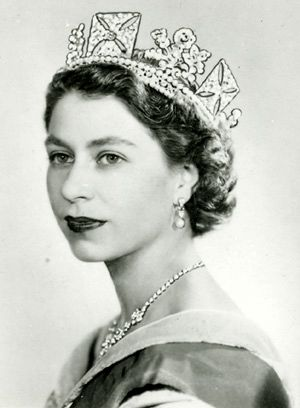
\includegraphics[width = 250px]{./picture/eli.jpg}
\end{center}

\end{figure}




\newpage

\tableofcontents

\newpage

\section{Introduction}

\vspace{1cm}

\subsection{Problématique et but du projet}

\vspace{1cm}

Dans le cadre du module de Programmation par Contraintes en Master 1 ALMA, nous avons eu pour objectif d'implémenter un solveur capable de résoudre le problème des \emph{N-Queens}. 

Ce projet est étendu sur trois séances, durant lesquelles nous avons dû concevoir ce solveur, capable d'effectuer une recherche complète des solutions, mais aussi une recherche locale, et enfin comparer les résultats d'exécutions sur des problèmes de taille variable.

Pour implémenter notre solveur, nous avons pris la décision d'utiliser le langage de Programmation Python3. Nous avons hésité avec $C++$, mais avons finalement choisi ce premier. Même si ses performances sont légèrement moins bonnes qu'avec $C++$, nous apprécions sa simplicité d’utilisation. De plus aucun autre module de notre Master ne nous a donné l’occasion de nous en servir, si bien que nous avons vu ici une opportunité pour nous réhabituer à ce langage particulièrement au goût du jour.

Dans ce rapport nous verrons en première partie le problème des \emph{N-Queens} avec plus de précision. Ensuite nous parlerons de la recherche complète que nous avons implémenté, puis la recherche locale. Enfin nous comparerons nous résultats d'exécution. 


\vspace{1cm}

\subsection{Problème des N-Queens}

Le problème des \emph{N-Queens} est un problème très célèbre dans le monde des mathématiques. Ce problème posé pour la première fois en 1850 par Franz Nauck consiste à trouver poser $n$ reines sur un échiquier faisant $n$ cases de côté sans qu'elles puissent s'attaquer. Ainsi elles ne doivent pas: 
\begin{itemize}
\item Etre sur la même ligne
\item Etre sur la même colonne
\item Etre sur la même diagonale
\end{itemize}

\\
Ce problème pose quelques problèmes, car il n'existe pas d'algorithme polynomial en complexité.


En testant toutes les possibilités de placement des reines sur un échiquier de taille 8*8 avec un algorithme de recherche exhaustive, on se retrouve à parcourir $64^8$ placements possibles, soit $2^4^8$, si bien qu'on arrive rapidement à des temps d'exécution bien trop longs. Néanmoins on peut réduire facilement ce temps d'exécution avec la programmation par contraintes. 
\newline

\subsubsection{Contraintes}

On doit ainsi modéliser les contraintes dans notre programme pour réduire drastiquement le nombre d'itérations avant de trouver une solution. Les contraintes, en langage naturel, sont donc:

\begin{itemize}
\item Il doit y avoir qu'une reine par ligne.
\item Il doit y avoir qu'une reine par colonne.
\item Il ne doit pas y avoir plus d'une reine par diagonale;
\end{itemize}

Ainsi pour modéliser ceci sous la forme d'un CSP, on utilisera les variables suivantes:
$x_i$: Reine de la ligne $i$.
$x_i = j$ : $j$, numéro de la colonne où est placée la reine.

Avec ce modèle on est sûr qu'il n'y aura pas d'attaques si deux reines sont sur la même ligne, puisqu'on ne permet qu'une seule reine par ligne.
Les contraintes sont donc les suivantes:
\begin{itemize}
\item Pas d'attaque sur les colonnes: $allDifferent(x_i)$ $\forall i \in [1, n]$. $\forall i \neq j$, $x_i \neq x_j$

\item Pas d'attaque sur les diagonales:  $\forall i \neq j, |x_i - x_j| \neq |i - j|$, et $\forall  1 \leq i < j \leq n : |x_i - x_j | \neq j - i$
\end{itemize}


\newpage
\subsection{Composition de notre groupe}

\vspace{1cm}

\begin{tabbing}


\=blaaaaaaaaaaaa\=bmaaaaaaaaaaaaaaaaaaaaaaaaa   \=baaaaaaa\kill \\
\>Thibault 	\>Béziers La fosse		\>M1ALMA\\
\>Dennis	\>Bordet			\>M1ALMA\\
\>Joachim	\>Clayton			\>M1ALMA\\
\>Alexis	\>Giraudet			\>M1ALMA\\
\>Benjamin 	\>Moreau			\>M1ALMA\\


\end{tabbing}

\vspace{1cm}
\section{Partie 1 : Complete Search}
\vspace{2cm}

\subsection {Définition}

Le Complete Search est une méthode qui vise à rechercher une solution au problème en parcourant un arbre de possibilité progressivement remplie.
Celui ci utilise un algorithms de backtracking.

\subsection{}



\vspace{1cm}
\section{Partie 2 : Local Search}
\vspace{2cm}

\subsection {Définition}

Le Local Search elle est une méthode qui 

\subsection {}


\vspace{1cm}
\section{Conclusion}
\vspace{2cm}


\end{document}
